\documentclass{tufte-handout}
\usepackage{amsmath}
\usepackage[utf8]{inputenc}
\usepackage{mathpazo}
\usepackage{booktabs}
\usepackage{microtype}

\usepackage{tikz}

\pagestyle{empty}


\title{Spanning USA}
\author{Lars Korduner \& Josefine Myllenberg}

\begin{document}
  \maketitle

  \section{Results}

  The following table summarizes our results:

  \bigskip\noindent
  \begin{tabular}{lr}
    \toprule
    Input file & MST total weight \\ \midrule
    USA-highway-miles.txt	 & 16598 \\
    tinyEWG-alpha.txt & 181 \\ \bottomrule
  \end{tabular}

  \bigskip
  The MST we found in tinyEWG-alpha.txt can be drawn like this:

  \medskip
  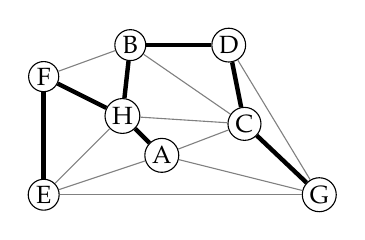
\begin{tikzpicture}[
      scale = .5,
      every node/.style = {
        circle, draw, black, inner sep = 1pt, font = \small},
      every path/.style = {gray}
      ]
    \node (A) at (3,1) {A}; % 0
    \node (B) at (2.2,3.8) {B}; % 1
    \node (C) at (5.1,1.8) {C}; % 2
    \node (D) at (4.7,3.8) {D}; % 3
    \node (E) at (0,0) {E}; % 4
    \node (F) at (0,3) {F}; % 5
    \node (G) at (7,0) {G}; % 6
    \node (H) at (2,2) {H}; % 7
    \draw (E)--(F);
    \draw (E)--(H);
    \draw (F)--(H);
    \draw (A)--(H);
    \draw (B)--(F);
    \draw (A)--(E);
    \draw (C)--(D);
    \draw (B)--(H);
    \draw (A)--(C);
    \draw (B)--(C);
    \draw (B)--(D);
    \draw (C)--(H);
    \draw (G)--(C);
    \draw (D)--(G);
    \draw (G)--(A);
    \draw (G)--(E);
    \begin{scope}[every path/.style={ultra thick}]
      \draw(A)--(H);
      \draw(H)--(F);
      \draw(F)--(E);
      \draw(B)--(H);
      \draw(B)--(D);
      \draw(D)--(C);
      \draw(C)--(G);
    \end{scope}
  \end{tikzpicture}


  \section{Implementation details}

  We implemented the algorithm of prim, using a adjacency list togeather with a priority queue.%

  The total running time for implementation is $O(mlogn)$.

\end{document}
